%
% File acl2017.tex
%
%% Based on the style files for ACL-2015, with some improvements
%%  taken from the NAACL-2016 style
%% Based on the style files for ACL-2014, which were, in turn,
%% based on ACL-2013, ACL-2012, ACL-2011, ACL-2010, ACL-IJCNLP-2009,
%% EACL-2009, IJCNLP-2008...
%% Based on the style files for EACL 2006 by 
%%e.agirre@ehu.es or Sergi.Balari@uab.es
%% and that of ACL 08 by Joakim Nivre and Noah Smith

\documentclass[11pt,a4paper]{article}
\usepackage[hyperref]{acl2017}
\usepackage{times}
\usepackage{latexsym}
\usepackage{bm}
\usepackage{graphicx}

\usepackage{url}

\aclfinalcopy % Uncomment this line for the final submission
%\def\aclpaperid{***} %  Enter the acl Paper ID here

%\setlength\titlebox{5cm}
% You can expand the titlebox if you need extra space
% to show all the authors. Please do not make the titlebox
% smaller than 5cm (the original size); we will check this
% in the camera-ready version and ask you to change it back.

\newcommand\BibTeX{B{\sc ib}\TeX}

\title{CS395T: Sequential CRF for NER Project Report}

\author{Zeyuan Hu \\
  Computer Science Department \\
  University of Texas at Austin \\
  Austin, Texas \\
  {\tt iamzeyuanhu@utexas.edu} \\
}

\date{}

\begin{document}
\maketitle

\begin{abstract}
In this project, I implement the Hidden Markove Model (HMM) and Conditional Random Field (CRF)
to solve the Parts-of-Speech tagging (POS) and the Named Entity Recognition (NER) problems
respectively. I extend the NER system with the beam search and the transition potential constraints.
A series of experiments show that the implementation of the system and the two extensions can have
significant impacts on the system performance.
\end{abstract}

\section{Collaborator}

\begin{itemize}
\item Zhan Shi {\tt zshi17@cs.utexas.edu}
\end{itemize}

\section{Introduction}

Parts-of-Speech (POS) tagging is a task to give a tag to each word in a given sentence.
Tag may include: noun, verb, pronoun, preposition, adverb, and so on. 
POS is important because knowing the tags of words can
give us the information about likely neighbouring words 
and the syntactic structure of the sentence,
which will be useful for Syntactic Parsing, Named Entity Recognition, and other 
information extraction tasks \cite[Chapter~10]{Jurafsky:2017}. However, since the amount
of tags and sentences can be large, manually tagging each words in a sentence
can be extremely time-consuming. Thus, we want to invoke some statistical model
to automatically generate the tags for us, which, in this case, is the Hidden Markov Model (HMM). 
I model the sequence of words and tags as markov chain
and use the maximum likelihood estimation to get the transition and emission probabilities.
Lastly, I use the Viterbi algorithm to infer the tags from the words sequence.

Another task I perform is the Named Entity Recognition (NER), which is about 
finding semantic components for a given sentence. For example, given a
sentence: "Barack Obama will travel to Hangzhou today for the G20 meeting.",
the NER system will generate the label "PERSON" for "Barack Obama", "LOC" for "Hangzhou" and "ORG" for "G20". 
The model I use for this task is the Conditional Random Field (CFR),
which I directly model the ouput labels $\boldsymbol{y}$ given the word sequence $\boldsymbol{x}$.
I use the forward-backward algorithm to train the model and use the Viterbi algorithm
to perform the inference of the labels.

\section{Implementation details}

\subsection{HMM}

For HMM, I implement the Viterbi algorithm. 
The code structure follows Figure 10.8 in \citet{Jurafsky:2017}. There
are two major parts: a initialization step and a recursion step. I implement two matrices
\verb|viterbi| and \verb|backpointer| with dimensions of $N$ by $T$, where
$N$ represents the number of tags(i.e., states) and $T$ represents the number of
words for a given sentence. \verb|viterbi| is used to keep track of the score for 
a given word and a given tag. \verb|backpointer| is used to store the optimium 
tags we have visited so far that maximize the score for the current tag given
the current word. In the initialization step, I calculate the score of each tag
for the first word and intitialize the values of \verb|backpointer| to be all zeros. In the recursion
step, I recursively calculate the score of each (tag,word) combination and keep track
of the optimum paths to each tag of the current word. Once we reach the final word, we can choose the tag that has the
highest score for the last word and then construct the best possible tag for each
word by recursively backtracking to the first word using the values stored 
in \verb|backpointer| matrix.

\subsection{CRF}

For the CRF, I implement the forward-backward
algorithm to train the model and the Viterbi algorithm for inference of the labels.
The Forward-backward algorithm allows us to compute $P(y_i = s|\boldsymbol{x})$,
which will be used in the Stochastic gradient descent (SGD) to update the weights of the model.
I use three matrices \verb|feature_matrix|, \verb|forward|, and \verb|backward| with dimensions
of $N$ by $T$ in my implementation. \verb|feature_matrix| is used to hold the calculation result
of $\phi_e(y_i,i,\boldsymbol{x})$. \verb|forward| and \verb|backward|
play the same roles as \verb|viterbi| matrix in HMM. The only differences between \verb|forward| and
\verb|backward| is how the score gets calculated: \verb|forward| calculates $\alpha_{i,t}$, whereas \verb|backward|
calculates $\beta_{i,t}$ \cite{Marsland:2014}. After forward-backward algorithm, I compute the gradient and
run the SGD to train the model. The implementation of the Viterbi algorithm in CRF is essentially
the same as the one in HMM. The only difference between these two versions is the extra constraints
on what labels sequence are considered valid in the CRF. The transition constraints
will be described in details in the next section.

\subsection{Extension}

My extension to the project is centered around the speed and the accuracy. 
For the speed, I implement the beam search for both HMM and CRF. 
For the accuracy, I encode hard constraints in the viterbi algorithm of the CRF
so that certain labels sequence will not get picked.
For the beam search, I maintain a list of \verb|beam|, which is a priority queue
that sorts the scores in the descending order. The implementation looks like
the Viterbi algorithm in the way that there are initialization and recursion steps as well. 
In the initialization
step, I set the beam for the first word and keep the labels that have the top \verb|beam_size|
scores. In the recursion step, for each label in the previous beam, I expand it
using $N$ labels and put the corresponding scores from the calculation 
into the current beam. At the last, we read through all the top of the beams to recover 
the best possible labels for the words sequence.

There are three types of labels sequence that are illegal in the NER system: 
1. We cannot have "O" label followed
by "I" label of any type (i.e., "O", "I-LOC"). 2. We cannot have two "I" labels with different
types next to each other (i.e., "I-LOC", "I-PER"). 3. We cannot have "I" label of a type that
is different from the "B" label's type that it follows (i.e., "B-LOC", "I-PER"). I handle all these
cases by explicitly checking these conditions in the recursion step of the Viterbi algorithm and
the beam search.

\section{Experiments}

Figure 1 shows the result of the F1 score of the NER system on the development set.
As the number of epoches in the trraining phase increases, the F1 scores increase 
but after around $15$ epoches, the F1 score becomes stable and stays above $85$. One extension to the system
is using the beam search instead of the Viterbi algorithm for the inference.
As shown in figure 1, the beam search has the same performance as the Viterbi algorithm
in terms of the F1 score. However, the beam search runs faster than the Viterbi algorithm.
A profiling of the system shows that 
the beam search with \verb|beam_size = 2| on average takes $2.18$ nanoseconds 
while the Viterbi algorithm takes $8.21$ nanoseconds for the same set of labels 
and sentences. 

\begin{figure}[bhp]
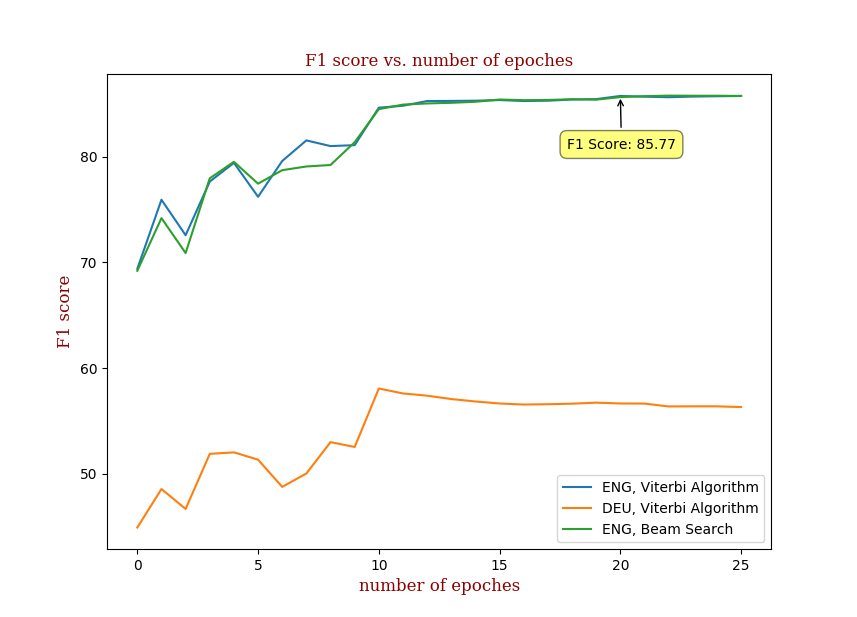
\includegraphics[width=\columnwidth]{F1.png}
\caption{F1 score vs. number of epoches in development set}
\end{figure}

Implementation of the system can have a huge impact on its performance as well. 
For example, I compare \verb|logsumexp| \cite{scipy} with \verb|logaddexp| \cite{scipy}
in the forward-backward score calculation. The former supports the vector input but the later
can only apply towards two numbers. I adopt the former in my inital implementation and
each epoch takes 150 seconds on average. Then, I experiment with the \verb|logaddexp| and find out
that each epoch takes 120 seconds on average while keeping the rest implementation untouched.
Another example is the learning rate of the SGD. I compare the constant $0.001$ learning rate
with a rate adjustment scheme of decreasing the rate by $10\%$ per $10$ iterations. 
The experiment shows that constant $0.001$ has a very slow convergence
to the global optimum: after five iterations, the F1 score is still below $70$. On the other hand,
the second scheme allows the system's F1 score to pass $80$ relatively quickly 
- around $15$ iterations. 

Encoding the transition potential constraints into both the Viterbi algorithm and
the beam search is the key factor in improving system labelling accuracy.
Without the transition potential constraints, the 
F1 score is capped at $83$ no matter the number of epoches used during the training phase.
The output of development set also confirms with the F1 scores as many sentences have 
been mislabeled with illegal labels sequence. After the integration of
the transition constraints into the algorithms, the F1 score rises to at least $85$ after around
$20$ epoches.

\section{Conclusion and Future Work}

In this project, I implement both the HMM and the CRF models for POS tagging and NER respectively. I
show the importance of function implementation choice and learning rate towards
the NER system performance. I add the beam search as 
an alternative inference algorithm for both HMM and CRF and the beam search
has the same performance as the Viterbi algorithm but with faster execution speed. 
In the future, the NER system can be further improved by exploring the potential performance gain
from the structured SVM instead of the CRF, using the AdaGrad optimizer instead of the SGD, and 
better feature engineering on the German NER data.

\bibliography{acl2017}
\bibliographystyle{acl_natbib}

\end{document}
